% Options for packages loaded elsewhere
\PassOptionsToPackage{unicode}{hyperref}
\PassOptionsToPackage{hyphens}{url}
%
\documentclass[
]{statsoc}
\usepackage{lmodern}
\usepackage{amssymb,amsmath}
\usepackage{ifxetex,ifluatex}
\ifnum 0\ifxetex 1\fi\ifluatex 1\fi=0 % if pdftex
  \usepackage[T1]{fontenc}
  \usepackage[utf8]{inputenc}
  \usepackage{textcomp} % provide euro and other symbols
\else % if luatex or xetex
  \usepackage{unicode-math}
  \defaultfontfeatures{Scale=MatchLowercase}
  \defaultfontfeatures[\rmfamily]{Ligatures=TeX,Scale=1}
\fi
% Use upquote if available, for straight quotes in verbatim environments
\IfFileExists{upquote.sty}{\usepackage{upquote}}{}
\IfFileExists{microtype.sty}{% use microtype if available
  \usepackage[]{microtype}
  \UseMicrotypeSet[protrusion]{basicmath} % disable protrusion for tt fonts
}{}
\makeatletter
\@ifundefined{KOMAClassName}{% if non-KOMA class
  \IfFileExists{parskip.sty}{%
    \usepackage{parskip}
  }{% else
    \setlength{\parindent}{0pt}
    \setlength{\parskip}{6pt plus 2pt minus 1pt}}
}{% if KOMA class
  \KOMAoptions{parskip=half}}
\makeatother
\usepackage{xcolor}
\IfFileExists{xurl.sty}{\usepackage{xurl}}{} % add URL line breaks if available
\IfFileExists{bookmark.sty}{\usepackage{bookmark}}{\usepackage{hyperref}}
\hypersetup{
  hidelinks,
  pdfcreator={LaTeX via pandoc}}
\urlstyle{same} % disable monospaced font for URLs
\usepackage{graphicx,grffile}
\makeatletter
\def\maxwidth{\ifdim\Gin@nat@width>\linewidth\linewidth\else\Gin@nat@width\fi}
\def\maxheight{\ifdim\Gin@nat@height>\textheight\textheight\else\Gin@nat@height\fi}
\makeatother
% Scale images if necessary, so that they will not overflow the page
% margins by default, and it is still possible to overwrite the defaults
% using explicit options in \includegraphics[width, height, ...]{}
\setkeys{Gin}{width=\maxwidth,height=\maxheight,keepaspectratio}
% Set default figure placement to htbp
\makeatletter
\def\fps@figure{htbp}
\makeatother
\setlength{\emergencystretch}{3em} % prevent overfull lines
\providecommand{\tightlist}{%
  \setlength{\itemsep}{0pt}\setlength{\parskip}{0pt}}
\setcounter{secnumdepth}{-\maxdimen} % remove section numbering
\title[ERGM and LOLOG Real-World Performance]{Comparing the Real-World Performance of Exponential-family Random Graph Models and Latent Order Logistic Models for Social Network Analysis}

% List abbreviations here, if any. Please note that it is preferred that abbreviations be defined at the first instance they appear in the text, rather than creating an abbreviations list.
% \abbrevs{LOLOG, latent order logistic model; ERGM, Exponential Random Graph Models; MCMC, Markov Chain Monte Carlo}

% Include full author names and degrees, when required by the journal.
% Use the \authfn to add symbols for additional footnotes and present addresses, if any. Usually start with 1 for notes about author contributions; then continuing with 2 etc if any author has a different present address.
\author[Duncan A. Clark]{Duncan A. Clark}
% \address{Duncan A. Clark, Department Of Statistics, University of California, Los Angeles, California, 90095}
\address{University of California - Los Angeles, Los Angeles, USA}
\email{duncanclark@ucla.edu}

\author[Mark S. Handcock]{Mark S. Handcock}
\address{University of California - Los Angeles, Los Angeles, USA}

% \presentadd[\authfn{2}]{Department, Institution, City, State or Province, Postal Code, Country}

% \fundinginfo{Put funding info here}

% Include the name of the author that should appear in the running header
% \runningauthor{Author One et al.}
\usepackage{amsmath}\usepackage{amsfonts}\usepackage{amssymb}\usepackage{mathrsfs}\usepackage{graphicx}\usepackage{float}\usepackage{url}\usepackage{epstopdf}\usepackage{booktabs}\usepackage{longtable}\usepackage{appendix}\usepackage[a4paper]{geometry}\usepackage{graphicx}\usepackage[textwidth=8em,textsize=small]{todonotes}\usepackage{amsmath}\usepackage{natbib}\usepackage{hyperref}\usepackage{xcolor}\usepackage{dsfont}\usepackage{colortbl}
\usepackage{booktabs}
\usepackage{longtable}
\usepackage{array}
\usepackage{multirow}
\usepackage{wrapfig}
\usepackage{float}
\usepackage{colortbl}
\usepackage{pdflscape}
\usepackage{tabu}
\usepackage{threeparttable}
\usepackage{threeparttablex}
\usepackage[normalem]{ulem}
\usepackage{makecell}
\usepackage{xcolor}

\author{}
\date{\vspace{-2.5em}}

\begin{document}

\newcommand{\R}{\mathbb{R}}
\newcommand{\N}{\mathbb{N}}
\newcommand{\E}{\mathbb{E}}
\newcommand{\V}{\mathbb{V}}
\newcommand{\bfR}{\mathbf{R}}
\newcommand{\bfX}{\mathbf{X}}
\newcommand{\bfW}{\mathbf{W}}
\newcommand{\bfD}{\mathbf{D}}
\newcommand{\INT}{\int_{-\infty}^{+\infty}}
\newcommand{\p}{\partial}
\newcommand{\ra}{\Rightarrow}
\newcommand{\dH}{d\mathscr{H}}
\newcommand{\ch}{\text{cosh}}
\newcommand{\sh}{\text{sinh}}
\newcommand{\ex}{\mathbb{E}\left[X\right]}
\newcommand{\ey}{\mathbb{E}\left[Y\right]}
\newcommand{\logit}{{\rm logit}}
\newcommand{\MOM}{{\rm MOM}}

\setcounter{secnumdepth}{4}

\begin{abstract}
Exponential-family Random Graph models (ERGM) are widely used in social network analysis when modelling data on the relations between actors. ERGMs are typically interpreted as a snapshot of a network at a given point in time or in a final state. The recently proposed Latent Order Logistic model (LOLOG) directly allows for a latent network formation process. We assess the real-world performance of these models when applied to typical networks modelled by researchers. Specifically, 
we model data from an ensemble of articles in the journal \textit{Social Networks} with published ERGM fits, and compare the ERGM fit to a comparable LOLOG fit. We demonstrate that the LOLOG models are, in general, in qualitative agreement with the ERGM models, and provide at least as good a model fit. In addition they are typically faster and easier to fit to data, without the tendency for degeneracy that plagues ERGMs.
Our results support the general use of LOLOG models in circumstances where ERGM are considered.
\end{abstract}
\keywords{Social Network Modelling, LOLOG, ERGM, Social Network Analysis, Degeneracy, Goodness-of-fit}

\section{Introduction}

Social network analysis has become increasingly important in recent
decades, with particular need in the social sciences to elucidate
relational structure \citep{Goldenberg2010}. However developing
generative models for social networks has proven challenging
\citep{chatterjee2013}. Here we consider a social network a collection
of fixed nodes, each with fixed covariates and with edges stochastically
present or absent between every pair of nodes. The chief problems for
modelling such data are the vast space of possible networks and probable
highly complex dependence structures of the network edges.

The Exponential-family Random Graph Models (ERGM) framework is widely
used to represent the stochastic process underlying social networks
\citep{FrankStrauss1986,Hunter2006}. ERGMs allow researchers to
quantitatively evaluate the impact of local social processes and nodal
attributes on the probability of edges between nodes forming. However
these models are prone to near-degeneracy \citep{Handcock2003} and can
not naively be applied to large networks
\citep{schweinberger2011,chatterjee2013}. Model degeneracy is the
application specific tendency of the model to concentrate probability
mass on a small subset of graphs, especially those which are not similar
to realistic networks for that application.

Much progress has been made on managing model degeneracy by introducing
local neighbourhood structures \citep{schweinbergerhandcock2015} or
tapering \citep{fellowshandcock2017}. The presence of degeneracy in many
fitted ERGMs motivates the search for alternative model classes with
similar or complementary modelling capacity that are less susceptible to
these challenges.

While ERGMs are descriptive, they are often embedded as the equilibrium
distribution of a social process. The Latent Order Logistic model
(LOLOG) \citep{Fellows2018} is a related model that uses an edge
formation process to develop a general probability model over the space
of graphs. It is motivated by using the so-called change statistics, the
change in the specified graph statistics resulting from toggling an edge
on or off, as predictors in a sequential logistic regression for each
possible edge. Noting that an ERGM specified with independent tie
variables, reduces to a sequential logistic regression on its change
statistics, ERGM and LOLOG are equivalent in the independent dyad case
\citep{Fellows2018}. LOLOG models also allow non-independent dyads, and
graph statistics that depend on the order of edge formation, which
result in different models than ERGM.

LOLOG models have the advantage that they are straightforward to sample
from, and can be used with simpler model terms, that would for an ERGM
almost certainly result in near-degeneracy. This allows for a fast and
user friendly fitting procedure, with easily interpretable model terms.

How can we assess and compare differing model classes? Both ERGM and
LOLOG are fully general and able to represent arbitrary distributions
over the set of graphs \citep[][Theorem 1]{Fellows2018}. As ERGMs are
the equilibrium distribution of a relatively general MCMC process, there
are many mechanisms that can lead to them, as there are for LOLOG. Hence
both model classes have strong theoretical and modelling motivations,
although the ERGM class to this point has been much more extensively
explored \citep{schweinberger2020,Schweinberger2017ExponentialFamilyMO}.
In this paper, we provide a separate and novel contribution to the
assessment on the model classes. Our objective is to compare the models
by a pairwise assessment on the population of networks that the research
community would choose to fit them on. The idea here is to move the
perspective from that of the model viewpoint (i.e., given we have a
model, what can we fit with it?) to a data-centric view point (i.e.,
given that this is the data we have, what are the best modelling
approaches?). The latter is the question facing the real-world users of
these models, while the``inverse problem'' addressed by the former is
commonly taken as it does not require the population of networks to be
specified.

However, to take the data-centric viewpoint, we need to specify the
population. We operationalised this in this paper by taking a population
of networks that ERGM models have been applied to in the premier journal
for publishing social network analyses, \textit{Social Networks}
\citep{socialnetworks}. \textit{Social Networks} is an interdisciplinary
journal for those with ``interest in the study of the empirical
structure of social relations and associations that may be expressed in
network form''. While the sub-population of networks in
\textit{Social Networks} for which ERGMs have been fit is a sample of
the population of interest, we believe that it is a salient and
(non-statistical) representative sub-population of the broader
population.

Our selection of ERGM papers was at first a census of papers in the
journal \textit{Social Networks} using the ERGM framework, published
from the journal's founding in 1979 up to and including the January 2016
issue. Note that we have chosen a population of networks that are biased
toward ERGM. These networks have successfully completed the peer-review
process of \textit{Social Networks}. In particular, the ERGM fit and
analyses have passed peer-review and are deemed of sufficient scientific
interest to appear in this premier journal. Clearly this is not
sufficient to ensure the fit and models are appropriate for the data,
although they represent a strong selectiveness relative to the
population of networks that researchers would consider for analysis
(without regard to a model class choice). Hence a comparable or
competitive fit for LOLOG models to this sub-population presents
stronger evidence for the value of LOLOG models than a comparison to the
broader population. In particular it seems likely that in papers
published that fit an ERGM model, ERGM performs well on this data set,
thus we expect a publication bias towards networks that suit ERGM well,
which may not necessarily suit LOLOG well. We therefore suggest that
good performance on data published with ERGM fits is a conservative
indicator that LOLOG is a useful model for analysing social networks.

Identifying, assembling and fitting ERGMs and LOLOGs to an ensemble of
networks, analysing their goodness of fit (GOF) and interpreting the
results, is a significant undertaking. For brevity we give the fit of
networks from a case-study \citep{Sailer2012} in detail and provide
summaries for the remaining networks in the supplement.

The structure of this paper is as follows. In Section \ref{sec:LOLOG} we
briefly introduce ERGMs and the LOLOG model, reviewing work in
\cite{Fellows2018} as well as discussing the theoretical similarities
and differences. Section \ref{sec:description} gives a description of
the ensemble of networks and discusses the motivation for selecting such
an ensemble. Section \ref{sec:offices} shows both the LOLOG and ERGM fit
of office layout networks with the data from \cite{Sailer2012}. Section
\ref{sec:results} presents a summary of all the LOLOG and ERGM fits to
each of the networks in the ensemble. Section \ref{sec:discussion}
discusses the results of the fitting, as well as its implications
regarding the utility of the LOLOG model.

\section{ERGM and LOLOG Model Classes}\label{sec:LOLOG}

Let \(Y\) be a random graph whose realisation is
\(y \in \mathscr{Y} = \lbrace a \in \mathbb{R}^{n \times n} \quad \vert \quad \forall i,j \quad y_{i,i} = 0 \quad y_{i,j} \in \lbrace 0,1 \rbrace\rbrace\).
We regard the number of nodes and any nodal covariates as fixed and
known. For undirected networks the additional restriction that
\(y_{i,j} = y_{j,i} \quad\forall i,j\) can be added. Let \(|y|=n(n-1)\)
denote the number of possible edges in \(y\) (\(|y|=n(n-1)/2\) for
undirected graphs). A dyad in a graph is a sub-graph of two nodes and
any ties between them.

\subsection{Model Specification}

LOLOG and ERGM are alternative specifications of the distribution of
\(Y\). An ERGM for the network can be expressed as
\begin{align}\label{eq:ERGM_spec}
p_{E}(y\vert \theta) = \frac{\exp(\theta\cdot g(y))}{c({\theta})}~~~~~ y\in \mathscr{Y}
\end{align} \noindent where \(g(y)\) is a \(d-\)vector valued function
defining a set of sufficient statistics; \(\theta \in \mathds{R}^{d}\)
is a vector of parameters; and \(c(\theta)\) the normalising constant.
Each ERGM family is defined by the choice of sufficient statistics.
These are chosen by the researcher, depending on domain knowledge, to
specify the generating social processes. They can be any statistical
summary of network properties and are typically motivated by social
theory \citep{goodkittsmorris09} or symmetry arguments \citep{str86}. In
this way, ERGMs constitute a family of models across different choices
of the sufficient statistics.\\
Typically graph statistics are the density and degree counts, as well as
nodal or edge covariate terms such as sociability and homophily
\citep{ergmtermsjss}. Geometrically weighed edgewise shared partner
(GWESP) and geometrically weighted degree (GWDEG) terms are often
included \citep{snijders2006} as they capture complex structure while
reducing the effects of near degeneracy \citep{Handcock2003}. A very
large number of terms are used by researchers in applications. Explicit
definitions of almost all terms used in this paper can be found in
\cite{ergmtermsjss} or the documentation of \cite{ergm_3_9_4}.
Regardless of which sufficient statistics are used, the ERGM will have
the maximal entropy of any distribution satisfying the \(d\)-dimensional
mean constraints placed on \(g(y), E[g(y)]=\mu\). LOLOG models posit the
existence of a latent discrete temporal dimension, \(t=1, \ldots, |y|\)
so that the edges form in a sequence. \cite{Fellows2018} defines the
latent random variables \(Y_{t},\ t=1, \ldots,\) representing the
sequential formation of \(Y.\) \(Y_{t}\) has exactly \(t\) edges and is
formed from \(Y_{t-1}\) by the addition of an edge. A LOLOG model is
specified by two components, The first is the probability of observing a
graph given a specified order of edge formation, \(s\): \begin{align}
p(y \vert s,\theta) &= \prod_{t=1}^{|y|} \frac{1}{Z_t(s)} \exp\left(\theta\cdot C_{s,t}\right)
\end{align} \noindent where
\(s=\{s_1, s_2, \ldots, s_{|y|}\} \in \mathscr{S}_{|y|}\) is the set of
possible edge formation orders with \(|y|\) dyads, and \begin{align}
C_{s,t} &= g(y_{t},s_{\leq t}) - g(y_{t-1},s_{\leq t-1})
\end{align} \noindent where \(s_{\leq t}\) denotes the first \(t\)
elements of \(s \in \mathscr{S}_{|y|}\). The \(C_{s,t}\) are the
difference in the graph statistics from the \(y_{t-1}\) network to the
\(y_{t}\) network and are informally called the ``change statistics'' of
the formation process. The \(Z_{t}(s)\) sequentially specify the
normalising constants. Let \(y_{t}^{+}\) be the graph \(y_{t-1}\) with
the edge \(s_{t}\) added, then \begin{align}
Z_{t}(s) &= \exp\left(g(y_{t}^{+},s_{\leq t}) - g(y_{t-1},s_{\leq t-1})\right) + 1
\end{align} The second component is the model for the edge order
permutations, \(p(s)\). The LOLOG distribution for \(Y\) is:
\begin{align}
p_{L}(y \vert \theta) &= \sum_{s} p(y \vert s, \theta)p(s) \nonumber \\
&= \sum_{s} \left( p(s)\prod_{t=1}^{|y|} \frac{1}{Z_t(s)} \exp\left(\theta\cdot C_{s,t}\right)\right) \label{eq:lolog}
\end{align}

\subsection{Model Interpretation}

For the LOLOG model, conditioning on an edge permutation \(s\), at each
step \(t\), we have
\({\rm logit}\left( {p(y_{t}^{+} \vert s_{\leq t}, y_{t-1}, \theta )}\right) = \theta\cdot C_{s,t}\).
Thus at each time \(t\), conditional on the network already formed by
that point, each dyad is a logistic regression on the change statistics
associated with the edge. For ERGMs, equation (\ref{eq:ERGM_spec})
yields the auto-logistic interpretation of the \(\theta\) parameter
\(\log\left(\frac{p(y_{i,j}^{+} \vert y_{i,j}^{c}, \theta )}{p(y_{i,j}^{-} \vert y_{i,j}^{c}, \theta )}\right) = \theta\cdot (g(y_{i,j}^{+}) - g(y_{i,j}^{-})),\)
where \(y_{i,j}^{c}\) is
\(y{\backslash}y_{i,j}, y_{i,j}^{+}=y_{i,j}^{c}\cup\{y_{i,j}=1\}\) and
\(y_{i,j}^{-} = y_{i,j}^{c}\cup\{y_{i,j}=0\}\). Thus, conditional on the
rest of the graph, each dyad can be thought of as an (auto)-logistic
regression on change statistics. This gives a helpful interpretation for
the parameters, but does not help interpret the probability distribution
of each edge unconditional of the rest of the graph.

\subsection{Model Estimation}

Due to the intractability of summing over all possible edge permutations
in the LOLOG model, the likelihood or likelihood ratio, cannot be
evaluated and the maximum likelihood estimate (MLE) is intractable.
\cite{Fellows2018} proposed a method of moments (MOM) approach to
estimate model parameters. The idea is to seek \(\theta_{{\rm MOM}}\)
such that
\(g(y) - \mathbb{E}_{\theta_{{\rm MOM}}}\left[ g(y) \right] = 0\).
\cite{Fellows2018} developed a Newton-Raphson approach as it is possible
to differentiate the
\(\mathbb{E}_{\theta_{{\rm MOM}}}\left[ g(y) \right]\) with respect to
\(\theta\) and approximate its value by sampling from the LOLOG model.
Along with introducing LOLOG models in \cite{Fellows2018}, the
\texttt{lolog} R package \citep{LOLOG_github} provides a sophisticated,
fast and user friendly method to fit LOLOG models to data.

ERGM parameters are typically estimated using an MCMC procedure to
estimate the MLE \citep{Snijders2002,Hunter2006}. This is
computationally demanding and there are sophisticated R packages
available to perform this estimation \citep{ergm_3_9_4}.

For both LOLOG and ERGM models we approximate standard errors derived
from MCMC estimated inverse Fisher information matrices.

\subsection{Model Discussion}\label{sec:comparison}

A key advantage of the LOLOG model is the ease of simulation from the
model. To simulate a network we simply draw \(s\) from \(p(s)\) and
perform a sequential logistic regression simulation on the change
statistics \citep{LOLOG_github}. The ERGM by comparison requires a full
MCMC procedure to simulate networks \citep{ergm_3_9_4}.

For LOLOG models we are required to model \(p(s)\) the probability mass
function (PMF) on the space of possible edge permutations. In the
absence of strong substantive reason for a particular partial ordering
of the edges, a uniform PMF can be used. However many natural reasons
exist to constrain the edge ordering. For example, in schools that
welcome a new cohort each year, edges in upper years could reasonably be
constrained to have been formed before edges in lower years.

For ERGMs the interpretation is conditional on the entire rest of the
network, whilst for LOLOG models with a specified edge ordering, the
interpretation is conditional only on the network formed up until that
point. We emphasise that the network formed up until that point will
depend on the particular edge permutation. We note that in the case
where the tie variables are independent, the edge ordering \(s\) does
not matter (as the dyads do not depend on each another) and LOLOG
reduces to logistic regression on change statistics, as does ERGM and to
the same model.

We may also compare dyad-dependent ERGM and LOLOG models through their
simulation algorithms A network from an ERGM is simulated through an
MCMC procedure where dyads are considered conditional on the rest of the
network. Often many thousands of steps are required to converge to the
stationary distribution. As noted above, the log odds is equal to the
inner product of the parameter and the change statistics of that dyad.
The LOLOG model is formed by first sampling a dyad ordering, then
starting with an empty network, adding an edge based on the log odds
(being the inner product of the parameter and the change statistic).
Each dyad is considered for edge formation and then the process is
terminated leaving the simulated graph.

LOLOG considers each dyad exactly once, whereas the ERGM process can
consider dyads multiple times for both edge formation and dissolution.
We suggest a reason that LOLOG models do not suffer from the same
degeneracy is that, in the simulation, each dyad is considered exactly
once. This limits the scope for the explosive edge formation or deletion
that often occurs when simulating from ERGM models.

More broadly we argue that the LOLOG, motivated as a model with an easy
simulation method with parameters that remain interpretable, is more
desirable than ERGMs even though the model is straightforward to write
down, but requires MCMC procedures to simulate from.

\subsection{Assessing Goodness of Fit}

For the interpretation of model parameters to be valid, we must show
that the model is a plausible generating process for the observed
network. In Section \ref{sec:offices} we follow the goodness of fit
procedure as in \cite{Hunter_Goodreau_2008}. That is, we graphically
compare the simulated distribution of chosen graph statistics to the
observed values of those graph statistics. Whilst our models are highly
parsimonious representations of complex social processes, the goodness
of fit method highlights, that at a minimum, we should expect the
observed statistics to be plausible realisations from a well fitting
model.

\section{Description of the Ensemble}\label{sec:description}

We considered papers in the journal \emph{Social networks} where ERGMs
were fit to data. We included papers up to and including the January
2016 issue. There were 45 such papers, of which we selected 18 papers as
follows. First, we excluded bipartite ERGMs (5), we then included all
networks with publicly available data (7) and selected a further 11
papers out of the remaining 33 based on their, subjectively assessed,
novelty as well as the likely availability and ability to share data. We
contacted the authors of the 11 papers and received the data for 7 of
the papers. This gave an ensemble of 137 networks in 14 peer reviewed
published papers, as many papers contained multiple networks. We note
that 102 of these networks were from a single paper \citep{Lubbers2007},
which were omitted from our analyses, leaving 35 networks. Table
\ref{tab:network_summaries} shows a brief summary for each of the
networks.

\begin{table}
\caption{\label{tab:network_summaries} Key properties of each network contained in the ensemble}\\
\begin{tabular}[t]{lllllr}
\toprule
Description & Network & Nodes & Edges & Directed  & Citation\\
\midrule
\rowcolor{gray!6}  Add Health &  & 1681 & 1236 & Undirected &  \cite{AddHealth2007}\\
\addlinespace
School Friends &  & Various & Varies & Directed &  \cite{Lubbers2007}\\
\rowcolor{gray!6}  Kapferer's Tailors &  & 39 & 267 & Undirected &  \cite{Robins2007}\\
\addlinespace
Florentine Families &  & 16 & 15 & Undirected &  \cite{Robins2007}\\
\rowcolor{gray!6}  German Schoolboys &  & 53 & 53 & Directed & \cite{Heidler2014}\\
\addlinespace
Employee Voice & 1 & 27 & 104 & Directed & \cite{Pauksktat2011}\\
\rowcolor{gray!6}  Employee Voice & 2 & 24 & 53 & Directed &  \cite{Pauksktat2011}\\
Employee Voice & 3 & 30 & 126 & Directed &  \cite{Pauksktat2011}\\
\rowcolor{gray!6}  Employee Voice & 4 & 31 & 139 & Directed &  \cite{Pauksktat2011}\\
Employee Voice & 5 & 37 & 149 & Directed &  \cite{Pauksktat2011}\\
\rowcolor{gray!6}  Employee Voice & 6 & 39 & 155 & Directed & \cite{Pauksktat2011}\\
\addlinespace
Office Layout & University & 67 & 211 & Directed & \cite{Sailer2012}\\
\rowcolor{gray!6}  Office Layout & University & 69 & 203 & Directed & \cite{Sailer2012}\\
Office Layout & Research & 109 & 458 & Directed & \cite{Sailer2012}\\
\rowcolor{gray!6}  Office Layout & Publisher & 119 & 872 & Directed & \cite{Sailer2012}\\
\addlinespace
Disaster Response &  & 20 & 148 & Directed & \cite{Doreian2012}\\
\addlinespace
\rowcolor{gray!6}  Company Boards & 2007 & 808 & 1997 & Undirected & \cite{Gygax2015}\\
Company Boards & 2008 & 808 & 1740 & Undirected & \cite{Gygax2015}\\
\rowcolor{gray!6}  Company Boards & 2009 & 808 & 1682 & Undirected & \cite{Gygax2015}\\
Company Boards & 2010 & 808 & 1622 & Undirected & \cite{Gygax2015}\\
\addlinespace
\rowcolor{gray!6}  Swiss Decisions & Nuclear & 24 & 282 & Directed & \cite{Fischer2015}\\
Swiss Decisions & Pensions & 23 & 294 & Directed & \cite{Fischer2015}\\
\rowcolor{gray!6}  Swiss Decisions & Foreigners & 20 & 169 & Directed & \cite{Fischer2015}\\
Swiss Decisions & Budget & 25 & 224 & Directed & \cite{Fischer2015}\\
\rowcolor{gray!6}  Swiss Decisions & Equality & 24 & 248 & Directed & \cite{Fischer2015}\\
Swiss Decisions & Education & 20 & 227 & Directed & \cite{Fischer2015}\\
\rowcolor{gray!6}  Swiss Decisions & Telecoms & 22 & 256 & Directed & \cite{Fischer2015}\\
Swiss Decisions & Savings & 19 & 138 & Directed & \cite{Fischer2015}\\
\rowcolor{gray!6}  Swiss Decisions & Persons & 26 & 280 & Directed & \cite{Fischer2015}\\
Swiss Decisions & Schengen & 26 & 316 & Directed & \cite{Fischer2015}\\
\addlinespace
\rowcolor{gray!6}  University Emails &  & 1133 & 10903 & Undirected & \cite{Toivonen2009}\\
\addlinespace
School Friends & grade 3 & 22 & 177 & Directed & \cite{Anderson1999}\\
\rowcolor{gray!6}  School Friends & grade 4 & 24 & 161 & Directed & \cite{Anderson1999}\\
School Friends & grade 5 & 22 & 103 & Directed & \cite{Anderson1999}\\
\addlinespace
\rowcolor{gray!6}  Online Links & Hyperlinks & 158 & 1444 & Directed & \cite{Ackland2011}\\
Online Links & Framing & 150 & 1382 & Undirected & \cite{Ackland2011}\\
\bottomrule
\end{tabular}
\end{table}

Our selection of ERGM papers was at first a census of papers in the
journal \textit{Social Networks} using the ERGM framework. The
conclusions drawn from this study should be considered stronger than if
the networks selected were sampled at random or through convenience. We
do note that we did take a selective sample as described above as a
first wave of networks to request data for, though this was also chosen
based on our thoughts on which networks the authors would be able and
willing to share.

We considered papers that used ERGMs for their statistical analyses as
the ERGM class of models is arguable the most widely used descriptive
statistical model for network analyses \citep{Amati2018}. Both LOLOG
models and ERGMs are typically used to model global network structure
using local network structure, thus comparing the two models is
appealing. While both LOLOG and ERGM can represent any given PMF over
the space of networks \citep{Fellows2018}, specifying interpretable
models that fit the data is often the practical challenge. There is no
obvious reason to suspect similar performance in terms of fit and
interpretability, when fit with similar network statistics, on the same
network. In particular it seems likely that in papers published that fit
an ERGM model, ERGM should perform well thus we expect a publication
bias towards networks that suit ERGM well compared to LOLOG. We
therefore suggest that good performance on data published with ERGM
fits, is a conservative indicator that LOLOG is a useful model for
analysing social networks.

We also note that the LOLOG model allows for the consideration of
information on the order of the edge formation within a network the
researcher may have. This is currently implemented by allowing edge
orderings to be constrained to those orderings compatible with the
sequential adding of nodes to the network, followed by the consideration
of all possible new edges. This is not possible in ERGM and few of the
available networks had plausible ordering mechanisms. However this may
not be entirely due to the lack thereof: without the ability to model
such an ordering process with ERGM, it seems likely that even if there
is a compelling sequential node adding process the data would not be
reported or even collected.

\section{Case Study of LOLOG and ERGM fits: Complex networks where ERGM is insufficient}\label{sec:offices}

In this section we consider a case study from a single published paper
where the networks in question are sufficiently complex to demonstrate
that ERGM can be insufficient and LOLOG can help in modelling social
network data.

We consider four networks of daily social interactions between workers
within four different office spaces. An ERGM based analysis was
originally carried out in \cite{Sailer2012}. Ties are present between
person \(i\) and person \(j\) if person \(i\) reported daily social
interaction with person \(j\). Two of the networks are of a British
university faculty before and after an office refurbishment, the
remaining two are a German research institute and a corporate publishing
company. The networks are directed and have 69, 63, 109 and 120
people/nodes, respectively.

The research question of interest in \cite{Sailer2012} was the effect of
spatial distance in the formation of social interactions within an
office environment. The authors specified an ERGM with terms to
represent the potential complex structure. These are listed in the first
column of Table 2 and detailed here. The edges term models the overall
propensity for social interactions, it has a similar role to an
intercept term in regression. The reciprocity term measures the
propensity for both people in a dyad to report social interaction with
the other. The GWESP term, with decay parameter 0.5, is an integrated
measure of the transitivity of social interactions
\citep[See][for a detailed
explanation]{snijders2006}. The Usefulness term is an edge-covariate
term, with value equal to the sum over edges of the usefulness measure:
for dyad \((i,j)\) being person \(i\)'s self reported perception of the
usefulness of person \(j\). It measures the direct dependence of the
propensity to have a social interaction on the usefulness of the person
nominated. The team match term is the number of ties between people from
the same team. It measures the propensity of teams to influence the
density of social interaction. floor match is similar to team match,
except it measures the importance of being on the same floor for social
interaction. The metric distance term is the sum of the shortest walking
distance in meters between the socially interacting peoples normal place
of work. Similarly, the topo distance is the sum of measures of how far
the desks could be perceived to be apart given the topography of the
office \citep[See][for precise definitions]{Sailer2012}. The
coefficients of the metric and topo distances measure the increase in
log-odds of a social interaction given the distance they are apart.
These coefficients are generally negative, indicating that social
interactions become less common as the distance increases.

The best fitting model was then selected using the Akaike Information
Criterion (AIC) and then a variety of different distance metrics were
added individually as edge-covariates. The best model in terms of AIC
was once again selected and analysed. Notably no analysis of the
goodness of fit for the models was provided.

\subsection{Model Fits}

\begin{table}

\caption{\label{tab:unnamed-chunk-2}\label{tab:sailer_ergm_pub} Office Layout ERGM fits as per the published results. In all cases the selected measure of distance is negative and significant suggesting that close office workers, are more likely to interact, even after allowing for team, floor, usefulness as well as social structure in the form of reciprocity and transitivity.}
\centering
\begin{threeparttable}
\begin{tabular}[t]{lllll}
\toprule
  & University 2005 & University 2008 & Research Institute & Publisher\\
\midrule
\rowcolor{gray!6}  Edges & -3.4 (0.37)*** & -4.41 (0.2)*** & -4.1 (0.12)*** & -5.07 (0.15)***\\
Reciprocity & 0.38 (0.45) & 0.62 (0.31)*** & 2.39 (0.2)*** & -1.26 (0.19)***\\
\rowcolor{gray!6}  GWESP(0.5) & 1.36 (0.14)*** & 1.24 (0.11)*** & 0.92 (0.07)*** & 2.09 (0.09)***\\
Usefulness & 0.7 (0.15)*** & 0.54 (0.11)*** & 0.81 (0.04)*** & 1.31 (0.05)***\\
\rowcolor{gray!6}  Team Match & 0.78 (0.18)*** & 0.56 (0.1)*** & NA & NA\\
\addlinespace
Floor Match & 0.15 (0.26) & 0.58 (0.14)*** & NA & NA\\
\rowcolor{gray!6}  Metric Distance & -0.04 (0.01)*** & -0.01 (0)*** & -0.01 (0)*** & NA\\
Topo Distance & NA & NA & NA & -0.06 (0)***\\
\bottomrule
\end{tabular}
\begin{tablenotes}
\item *** p-value < 0.001 , ** p-value < 0.01, * p-value < 0.05
\end{tablenotes}
\end{threeparttable}
\end{table}

We were able to recreate the selected ERGM fit for all four networks,
shown in Table \ref{tab:sailer_ergm_pub}. The reciprocity coefficient is
positive in two of the networks, indicating that the conditional
log-odds of a social interaction is positive if the social interaction
is mutual. The GWESP coefficient is positive for all four networks,
indicating that the log-odds of a social interaction existing is
positive if the social interaction increases this measure of
transitivity. The usefulness coefficient is positive for all four
networks, indicating that the log-odds of a social interaction existing
is positively related to the usefulness of the nominated person. The
team match coefficient is positive for all four networks, indicating
that the log-odds of a social interaction existing is positive if the
social interaction is within the same team (as distinct from between
people in different teams). Floor match coefficients are also positive,
indicating that the log-odds of a social interaction existing is
positive if the social interaction is within the same floor (as distinct
from between people in different floors). The metric and topo
coefficients are generally negative, indicating that social interactions
become less common as the distance increases.

Overall, the \cite{Sailer2012} concluded that daily social interactions
of people in offices exhibit a tendency for mutuality and social
closure. Interactions are also more likely to occur where there is a
high level of usefulness of the receiver to the sender as well as within
teams. While being on the same floor plays a role in some cases, the
distance apart plays a role in all cases, with social interactions more
likely for people closer together.

We were able to obtain LOLOG fits with the same covariates, as the ERGM
fits for all networks, we summarise the fits in Table
\ref{tab:sailer_lolog_pub}. In addition we show the LOLOG fit using
GWESP, 2- and 3- in- and out-stars, together with all covariate matches
and metric distance in Table \ref{tab:sailer_lolog_gwesp_star}. For
\(k=1, 2, \ldots,\) a \(k\)-in-star centred on a node \(i\) and a set of
\(k\) different nodes \(\{i_1, \ldots, i_{k}\}\) such that the tie from
\(i\) to \(i_{j}\) exists for \(j=1, \ldots, k\). The \(k\)-in-star
statistic is the number of distinct \(k\)-in-stars in the network (i.e.,
summing over the centring nodes). The \(k\)-out-star statistic is the
same except the ties from \(i_{j}\) to \(i\) must exist for
\(j=1, \ldots, k\) (rather than the in-ties to \(i\)). As noted in
Section 2.2, the qualitative interpretation of the LOLOG coefficients is
similar to ERGM with the primary difference being the log-odds is
conditional on the network at the point the edge is added. We directly
compare the qualitative fits in Section 4.3.

\begin{table}

\caption{\label{tab:unnamed-chunk-3}\label{tab:sailer_lolog_pub}Office Layout LOLOG fit with same terms as published ERGM. Shows broad quantitative agreement with the published results using ERGM in Table \ref{tab:sailer_ergm_pub}}
\centering
\begin{threeparttable}
\begin{tabular}[t]{lllll}
\toprule
  & University 2005 & University 2008 & Research Institute & Publisher\\
\midrule
\rowcolor{gray!6}  Edges & -1.69 (0.38)*** & -3.67 (0.36)*** & -3.18 (0.13)*** & -1.63 (0.09)***\\
Reciprocity & 1.99 (0.34)*** & 1.96 (0.31)*** & 3.9 (0.25)*** & 0.64 (0.2)***\\
\rowcolor{gray!6}  GWESP(0.5) & 0.55 (0.12)*** & 0.87 (0.13)*** & 0.73 (0.09)*** & -0.22 (0.06)***\\
Usefulness & 1.02 (0.15)*** & 0.81 (0.14)*** & 1.21 (0.05)*** & 1.89 (0.06)***\\
\rowcolor{gray!6}  Team Match & 1.29 (0.19)*** & 0.72 (0.19)*** & NA & NA\\
\addlinespace
Floor Match & -0.28 (0.3) & 1.08 (0.29)*** & NA & NA\\
\rowcolor{gray!6}  Metric Distance & -0.07 (0.01)*** & -0.02 (0.01)*** & -0.02 (0)*** & NA\\
Topo Distance & NA & NA & NA & -0.1 (0)***\\
\bottomrule
\end{tabular}
\begin{tablenotes}
\item *** p-value < 0.001 , ** p-value < 0.01, * p-value < 0.05
\end{tablenotes}
\end{threeparttable}
\end{table}

\begin{table}

\caption{\label{tab:unnamed-chunk-4}\label{tab:sailer_lolog_gwesp_star}
      Office Layout LOLOG fit with GWESP and 2- and 3- in- and out-stars. Significant out-star terms may suggest there is social structure unaccounted for with just the published ERGM terms. Despite additional significant structural terms, still shows broad quantitative agreement with the published results using ERGM}
\centering
\begin{threeparttable}
\begin{tabular}[t]{lllll}
\toprule
  & University 2005 & University 2008 & Research Institute & Publisher\\
\midrule
\rowcolor{gray!6}  Edges & -3.2 (0.67)*** & -5.04 (0.59)*** & -4.04 (0.22)*** & -4.87 (1.19)***\\
Reciprocity & 2.03 (0.77)*** & 1.11 (0.45)*** & 4.7 (0.52)*** & 3.16 (1.27)***\\
\rowcolor{gray!6}  GWESP(0.5) & 0.33 (0.2) & 0.49 (0.16)*** & 0.77 (0.11)*** & 0.01 (0.26)\\
Out-2-Star & 1.39 (0.26)*** & 0.65 (0.16)*** & 0.41 (0.07)*** & 0.69 (0.15)***\\
\rowcolor{gray!6}  Out-3-Star & -0.28 (0.07)*** & -0.07 (0.03)*** & -0.04 (0.01)*** & -0.02 (0)***\\
\addlinespace
In-2-Star & 0.26 (0.22) & 0.25 (0.15) & 0.21 (0.12) & 0.73 (0.54)\\
\rowcolor{gray!6}  In-3-Star & -0.04 (0.05) & -0.03 (0.02) & -0.09 (0.03)*** & -0.18 (0.1)\\
Usefulness & 1.07 (0.2)*** & 0.75 (0.16)*** & 1.28 (0.07)*** & 2.98 (0.61)***\\
\rowcolor{gray!6}  Team Match & 1.93 (0.31)*** & 1.14 (0.25)*** & NA & NA\\
Floor Match & -0.24 (0.47) & 1.35 (0.43)*** & NA & NA\\
\addlinespace
\rowcolor{gray!6}  Metric Distance & -0.09 (0.01)*** & -0.02 (0.01)*** & -0.02 (0)*** & NA\\
Topo Distance & NA & NA & NA & -0.24 (0.06)***\\
\bottomrule
\end{tabular}
\begin{tablenotes}
\item *** p-value < 0.001 , ** p-value < 0.01, * p-value < 0.05
\end{tablenotes}
\end{threeparttable}
\end{table}

We were also able to fit LOLOG models to each of the networks when the
GWESP term is replaced with a triangle term. This is not possible with
ERGM due to near-degeneracy. We summarise this in Table
\ref{tab:sailer_lolog_tri}. The estimated standard errors for the
Publisher network are very high, suggesting there is great uncertainty
in the data generating process. The estimated standard errors for the
mutual and triangle terms for the University in 2005 and 2008 are also
high though not as severe and they fall out of significance for these
model fits. As the triangle term increases the estimated standard errors
and does not improve the GOF (see next section), we suggest using the
GWESP term.

We also fitted the LOLOG model where the people are added in the order
of their average usefulness, as reported by the other people. As we
suspect more useful people may have been in the office longer or should
be the first point of contact for new employees we suggest this as a
plausible ordering mechanism. The fit was comparable to the fit without
the ordering, and the GOF was not improved, so we do not consider it
further.

We tried to fit an ERGM model with the in- and out- geometrically
weighted degree (GWDEG) terms but this was degenerate for the University
2005 and 2008 networks. The in-GWDEG term adds one network statistic to
the model equal to a weighted sum of the in-degree counts with weights
decreasing geometrically. The out-GWDEG is similar with the out-degree
counts \citep[See][for a detailed explanation]{hunter07}. For the
Research institute and Publisher out-GWDEG was negative and significant,
in line with the LOLOG model positive 2-star and negative 3-star
parameters. However, the fit was still poor and inferior to the LOLOG
model. We do not comment further on this, though it is reassuring that
the ERGM with GWDEG gives similar interpretations to LOLOG with star
terms. The GWDEG terms were not discussed in \cite{Sailer2012}.

We note the computation time difference in the LOLOG and ERGM parameter
estimation. We ran each with a single core with Intel(R) Xeon(R)
Platinum 8160 CPU @ 2.10GHz processor. The recreated ERGM took around 35
seconds, and the LOLOG took around 8 seconds. For larger networks, we
found parallelisation in the network simulation step of the fit to be
extremely helpful for both the LOLOG and ERGM models. From our
experience for larger networks the performance differential between
LOLOG and ERGM can be much greater, in particular when the ERGM MCMC
simulation is computationally expensive.

\begin{table}

\caption{\label{tab:unnamed-chunk-5}\label{tab:sailer_lolog_tri} Office Layout LOLOG fit with triangles instead of gwesp term, hows broad quantitative agreement with the published results on nodal covariates, however suggests little tendency for reciprocity and transitivity in the university networks.}
\centering
\begin{threeparttable}
\begin{tabular}[t]{lllll}
\toprule
  & University 2005 & University 2008 & Research Institute & Publisher\\
\midrule
\rowcolor{gray!6}  Edges & -2.05 (0.82)*** & -3.9 (0.67)*** & -3.36 (0.15)*** & -5.4 (49.3)\\
Reciprocity & -2.96 (5.83) & -0.08 (1.6) & 3.34 (0.36)*** & -24.8 (367.3)\\
\rowcolor{gray!6}  Triangles & 2.69 (2.95) & 1.2 (0.73) & 0.61 (0.13)*** & 3.71 (50.63)\\
Usefulness & 1.35 (0.53)*** & 0.83 (0.16)*** & 1.21 (0.06)*** & 6.57 (88.39)\\
\rowcolor{gray!6}  Team Match & 1.8 (0.85)*** & 0.9 (0.35)*** & NA & NA\\
\addlinespace
Floor Match & -0.29 (0.88) & 1.07 (0.46)*** & NA & NA\\
\rowcolor{gray!6}  Metric Distance & -0.1 (0.05)*** & -0.02 (0.01)*** & -0.02 (0)*** & NA\\
Topo Distance & NA & NA & NA & -0.39 (5.82)\\
\bottomrule
\end{tabular}
\begin{tablenotes}
\item *** p-value < 0.001 , ** p-value < 0.01, * p-value < 0.05
\end{tablenotes}
\end{threeparttable}
\end{table}

\subsection{Goodness of Fit}

Firstly we consider the goodness of fit for the published ERGM model,
and the LOLOG model with the same terms. Figures
\ref{fig:sailer_gof_pub_ideg} show the comparison of simulated
distribution of the in-degree with the observed network statistics.
Figures \ref{fig:sailer_gof_pub_odeg} and \ref{fig:sailer_gof_pub_esp}
contained in Appendix \ref{app:GOF} show the same comparison for ESP and
out-degree.

\begin{figure}

{\centering 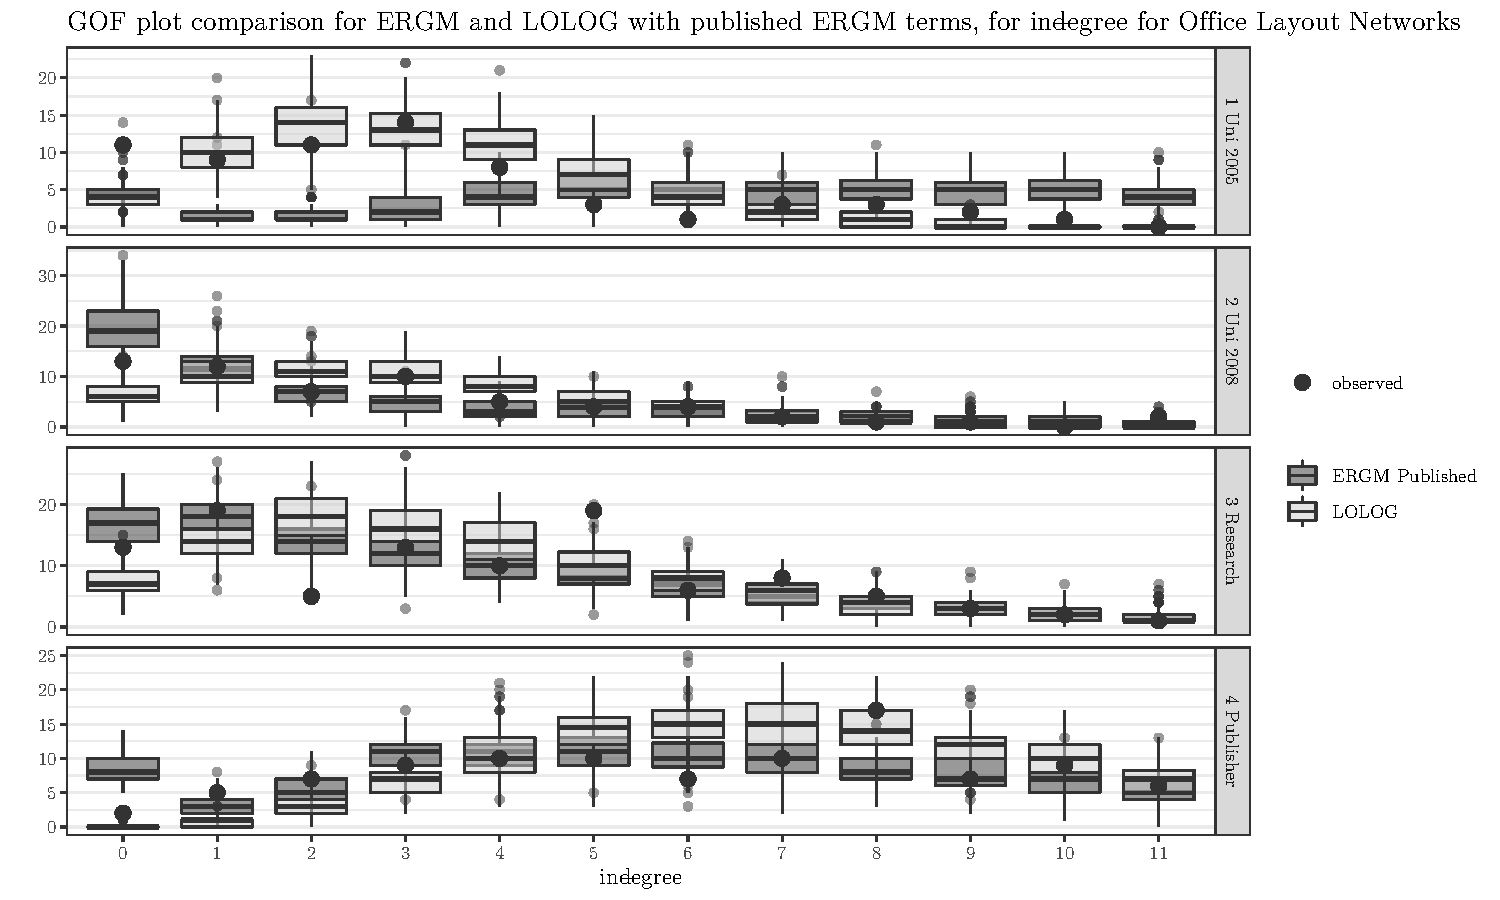
\includegraphics{lolog_catelog_writeup_JRSSA_major_revisions_git_files/figure-latex/unnamed-chunk-6-1} 

}

\caption{\label{fig:sailer_gof_pub_ideg}Sailer's Offices ERGM and LOLOG model with published terms, in-degree Goodness of Fit}\label{fig:unnamed-chunk-6}
\end{figure}

Table \ref{tab:GOF_comment_table} shows comments on the goodness of fit
for each network, using the recreated published ERGM and the LOLOG model
with published ERGM terms. Where no comment is made for any of the
goodness of fit terms or any model, the model fits well on that
statistic.

\begin{table}
\caption{Summary of GOF for ERGM and LOLOG with published terms for Office Layout networks. For all networks neither the LOLOG model or ERGM provide satisfactory fit.}
\label{tab:GOF_comment_table}
\begin{tabular}{@{}lll@{}}
\toprule
Network            & ERGM                                                                                                 & LOLOG                                                                                                                                                           \\ \midrule
\rowcolor{gray!6}
2005 University    & \begin{tabular}[c]{@{}l@{}}Fits poorly on out-degree\\ Fits poorly on ESP\end{tabular}                & \begin{tabular}[c]{@{}l@{}}Fits poorly on in-degree\\ Fits poorly on ESP but much better than ERGM\end{tabular}                     \\ \hline
2008 University    &      \begin{tabular}[c]{@{}l@{}}Fits poorly on out-degree\\ Fits poorly on ESP\end{tabular}                                                                                                 & \begin{tabular}[c]{@{}l@{}} ERGM convex, LOLOG concave on in-degree\\ Fits poorly on out-degree\\ Fits poorly on ESP\end{tabular} \\\hline
\rowcolor{gray!6}
Research Institute & \begin{tabular}[c]{@{}l@{}}Fits poorly on out-degree\\ Fits poorly on ESP \end{tabular}                                                                                         & \begin{tabular}[c]{@{}l@{}}Fits poorly on in-degree \\ Fits poorly on out-degree \\ Fits poorly on ESP \end{tabular}                                                                                                                                              \\\hline
Publisher          & \begin{tabular}[c]{@{}l@{}}Fits poorly on in-degree \\ Fits poorly on out-degree\\ Fits poorly on ESP\end{tabular} & \begin{tabular}[c]{@{}l@{}}Fits poorly on in-degree\\ Fits poorly on out-degree\\ Fits poorly on ESP\end{tabular}                                               \\ \bottomrule
\end{tabular}
\end{table}

All models for all networks have a least one of the in-degree,
out-degree or ESP statistic of the observed network not being a typical
value for the fitted models. As a result the models do poorly on
recreating networks similar to the observed, and thus inference based on
the parameter estimates and standard errors should be treated with
caution. In particular we note that the LOLOG model with identical terms
to the published ERGM does not seem to help improve the fit for any of
the networks in question here.

We also show the GOF for in-degree the LOLOG model with GWESP and 2- and
3- in- and out-stars for each model in Figure
\ref{fig:sailer_gof_gwesp_star_ideg}. Figures
\ref{fig:sailer_gof_gwesp_star_odeg} and
\ref{fig:sailer_gof_gwesp_star_esp} contained in Appendix \ref{app:GOF}
show the plots for out-degree and ESP. We note here that all models fit
the in-degree distribution well, all models except for the Publisher
network fit the out-degree distribution well and the University 2005 and
2008 models fit well on the ESP distribution. This is an improvement in
all cases versus the ERGM models published in \cite{Sailer2012}.

\begin{figure}
\centering
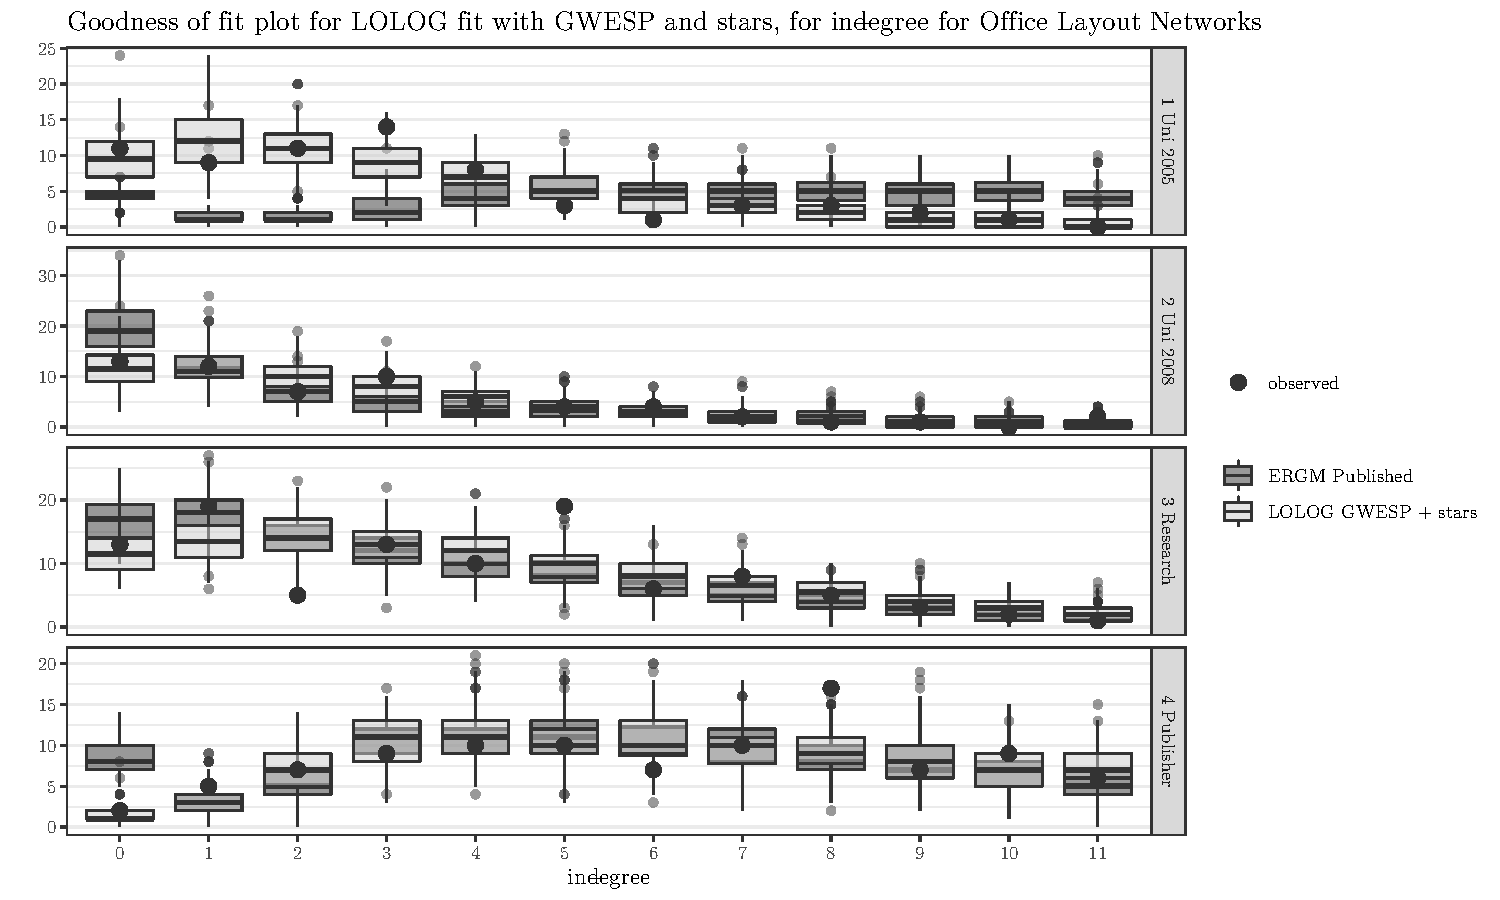
\includegraphics{lolog_catelog_writeup_JRSSA_major_revisions_git_files/figure-latex/unnamed-chunk-7-1.pdf}
\caption{\label{fig:sailer_gof_gwesp_star_ideg}Sailer's Offices LOLOG
model with GWESP and stars, in-degree Goodness of Fit}
\end{figure}

\subsection{Model Comparison}

These networks are of particular interest as they represents a real
world cases of applied researchers seeking a statistical tool to
represent and test their social hypotheses and analyse their collected
data. Good performance in such settings for the LOLOG model suggests the
model could be of real use to the applied social network research
community. Using these four complex networks as an example, helps us to
present the the utility of the LOLOG model. The ERGM and LOLOG models
with the terms as in \cite{Sailer2012} produced the same qualitative
interpretation.

However it is important to note that neither the specific LOLOG or the
ERGM fitted the data well in terms of all in-degree, out-degree and ESP
distributions. Therefore the models are not capturing basic aspects of
the observed network data and the above interpretation should be treated
with caution. In particular the Publisher network proved especially hard
to fit.

Using the triangle term in the LOLOG model in place of the GWESP term
did not improve the fit. Including 2- and 3- in- and out-star terms
yields models that fit much better on the in- and out-degree
distribution as well and the ESP distribution. We therefore have more
belief that inferences from these models are valid. They show similar
conclusions to the published ERGM, though in addition we observe a
significant positive out-2-star coefficient and a significant negative
out-3-star coefficient, suggesting that there is a tendency for some
people to have social interactions with many more people that others.
This tendency for super-daily interactors was not captured in the
published ERGM fit. We also note that the lack of a significant
in-2-star parameter suggests that there is not a corresponding tendency
for some people to attract more interactions, when their usefulness had
already been accounted for. We can infer that perhaps there is a surplus
of unwanted daily interaction due to people with a tendency for high
out-degree. Thus the LOLOG model allowed for a better fit, as well as a
deeper interpretation of the social interaction process.

\section{Summary of Results for the Ensemble}\label{sec:results}

The comparison of the value of models rarely will come down to a
quantitative measure on a single dimension. The social processes that
produce network data are typically complex and our choice of which data
to analyse tends to favour complex structures. The models typically only
approximate that structure and some features of the data are not
represented in the models. Scientists that model social network data
typically have multiple objectives with some models more suited to some
of those objectives rather than others. Having said this, we constructed
a rubric of criteria to assess the models, both relatively and
absolutely. We follow each criterion with a brief justification for why
it was included.

\begin{enumerate}
\item Are we able to recreate the published ERGM qualitatively?\\
We asked this to screen out network data where our usage differs qualitatively from the original, for whatever reason. This is to help ensure we were using the data correctly, so that our comparison is valid.
\item Do the recreations of the published ERGM fit the network well?\\
This is to assess the validity of the published ERGM results, and to assess if ERGM is a good model for the published case study.
\item Are we able to fit the LOLOG with the published ERGM terms?\\
This is to assess the LOLOG on terms likely favourable to the ERGM. Typically, published ERGM will have undergone model selection criteria to
choose terms that had good fit compared to other possible ERGM. This criteria assesses the flexibility of the LOLOG model class.
\item Does the LOLOG model with the published ERGM terms fit well?\\
This is an absolute measure of the LOLOG goodness-of-fit with the ERGM terms.
\item Are we able to fit the LOLOG model with ERGM Markov terms (that are often degenerate in ERGM)?\\
Markov terms, such as $k$-stars and triangles, often lead to near-degenerate models despite their conceptual appeal \citep{FrankStrauss1986}. This criteria assesses if the LOLOG can aid in interpretability by using simpler terms that are not possible in ERGM.
\item Is a better fit achieved with LOLOG than the published ERGM?\\
This is a direct comparison to judge if the LOLOG is a better model for the observed data than the published ERGM.
\item Do the published ERGM and best-fitting LOLOG models have consistent interpretations?\\
This assesses if qualitative substantive conclusions draw from each model are consistent with the other.
If affirmative, this gives some confidence that qualitative conclusions are not simply an artifact of the chosen modelling approach.
\item Which model do we believe to be more useful?\\
This is a subjective judgement criterion. A major component is the goodness-of-fit criteria (Section 2.5). These criteria measure the degree that important statistical characteristics of the network data are reproduced by the model. These focus on characteristics not explicitly in the model. A second component is the substantive interpretability of the terms (i.e., are they socially salient). A third is the complexity of the model terms (i.e., the value of simplicity).
\end{enumerate}

Table \ref{tab:summary_table} provides a summary of the ERGM and LOLOG
model fits for the networks in our ensemble, the columns are binary
answers (1=Yes, 0 = No), to the above criteria. The fits were carried
out in R using the \texttt{ergm} package \citep{ergm_3_9_4}, and the
\texttt{lolog} package \citep{LOLOG_github}. For the GWESP, GWDSP and
GWDEG terms decay parameters were used as stated. If they where not
available, \(\alpha= 0.5\) was used.

\begin{table}
\caption{\label{tab:summary_table} Summary table for LOLOG and ERGM Fits}\\
\begin{tabular}[t]{lllllllllll}
\toprule
Description & Network & Nodes & a & b & c & d & e & f & g & h\\
\midrule
\rowcolor{gray!6}  Add Health &  & 1618 & 1 & 0 & 1 & 0 & 1 & 1 & 1 & LOLOG\\
School Friends &  & Various &  &  &  &  &  &  &  & \\
\rowcolor{gray!6}  Kapferer's Tailors &  & 39 & 1 & 0 & 1 & 0 & 1 & 1 & 0 & LOLOG\\
Florentine Families &  & 16 & 1 & 1 & 1 & 1 & 1 & 1 & 0 & ERGM\\
\rowcolor{gray!6}  German Schoolboys &  & 53 & 1 & 1 & 0 & NA & 1 & 1 & 1 & Both\\
\addlinespace
Employee Voice & 1 & 27 & 0 & NA & 1 & 1 & 1 & 1 & NA & LOLOG\\
\rowcolor{gray!6}  Employee Voice & 2 & 24 & 1 & 1 & 0 & NA & 0 & 0 & NA & ERGM\\
Employee Voice & 3 & 30 & 0 & NA & 1 & 1 & 1 & 1 & NA & LOLOG\\
\rowcolor{gray!6}  Employee Voice & 4 & 31 & 0 & NA & 1 & 1 & 1 & 1 & NA & LOLOG\\
Employee Voice & 5 & 37 & 0 & NA & 1 & 1 & 1 & 1 & NA & LOLOG\\
\addlinespace
\rowcolor{gray!6}  Employee Voice & 6 & 39 & 0 & NA & 1 & 1 & 1 & 1 & NA & LOLOG\\
Office Layout & University & 67 & 1 & 0 & 1 & 0 & 1 & 1 & 1 & LOLOG\\
\rowcolor{gray!6}  Office Layout & University & 69 & 1 & 1 & 1 & 0 & 1 & 1 & 1 & LOLOG\\
Office Layout & Research & 109 & 1 & 1 & 1 & 0 & 1 & 1 & 1 & LOLOG\\
\rowcolor{gray!6}  Office Layout & Publisher & 119 & 1 & 0 & 1 & 0 & 1 & 1 & 1 & LOLOG\\
\addlinespace
Disaster Response &  & 20 & 0 & 0 & 0 & 0 & 1 & 1 & 0 & LOLOG\\
\rowcolor{gray!6}  Company Boards & 2007 & 808 & 0 & 0 & 0 & 0 & 1 & 1 & NA & LOLOG\\
Company Boards & 2008 & 808 & 0 & 0 & 0 & 0 & 1 & 1 & NA & LOLOG\\
\rowcolor{gray!6}  Company Boards & 2009 & 808 & 0 & 0 & 0 & 0 & 1 & 1 & NA & LOLOG\\
Company Boards & 2010 & 808 & 0 & 0 & 0 & 0 & 1 & 1 & NA & LOLOG\\
\addlinespace
\rowcolor{gray!6}  Swiss Decisions & Nuclear & 24 & 0 & 1 & 0 & NA & 1 & 1 & 1 & ERGM\\
Swiss Decisions & Pensions & 23 & 0 & 1 & 1 & 0 & 1 & 0 & 0 & ERGM\\
\rowcolor{gray!6}  Swiss Decisions & Foreigners & 20 & 0 & 1 & 0 & NA & 1 & 0 & 0 & ERGM\\
Swiss Decisions & Budget & 25 & 0 & 1 & 0 & NA & 1 & 1 & 0 & ERGM\\
\rowcolor{gray!6}  Swiss Decisions & Equality & 24 & 0 & 0 & 0 & NA & 1 & 1 & 0 & LOLOG\\
\addlinespace
Swiss Decisions & Education & 20 & 0 & 0 & 1 & 0 & 1 & 1 & NA & LOLOG\\
\rowcolor{gray!6}  Swiss Decisions & Telecoms & 22 & 0 & 0 & 0 & NA & 1 & 1 & NA & LOLOG\\
Swiss Decisions & Savings & 19 & 1 & 1 & 0 & NA & 1 & 1 & 0 & ERGM\\
\rowcolor{gray!6}  Swiss Decisions & Persons & 26 & 0 & 1 & 0 & NA & 1 & 1 & 0 & ERGM\\
Swiss Decisions & Schengen & 26 & 0 & 0 & 0 & 0 & 1 & 1 & NA & LOLOG\\
\addlinespace
\rowcolor{gray!6}  University Emails &  & 1133 & 0 & 0 & 0 & 0 & 0 & 0 & NA & Neither\\
School Friends & grade 3 & 22 & 1 & 0 & 0 & 0 & 1 & 1 & NA & LOLOG\\
\rowcolor{gray!6}  School Friends & grade 4 & 24 & 1 & 0 & 0 & 0 & 1 & 1 & NA & ERGM\\
School Friends & grade 5 & 22 & 1 & 0 & 0 & 0 & 1 & 1 & NA & ERGM\\
\rowcolor{gray!6}  Online Links & Hyperlinks & 158 & 1 & 0 & 1 & 0 & 1 & 1 & 1 & LOLOG\\
\addlinespace
Online Links & Framing & 150 & 1 & 0 & 1 & 0 & 1 & 0 & 1 & LOLOG\\
\hline
\hline
\rowcolor{gray!6}  Column Proportion & NA & NA & 0.43 & 0.37 & 0.46 & 0.23 & 0.94 & 0.86 & 0.5 & NA\\
\bottomrule
\end{tabular}
\end{table}

Finally, we make some general comments regarding the significant amount
of information on the hundreds of models fitted to the data that we
gathered, more detailed summaries for each individual network are
contained the supplement. More detailed overall comments on the study
are in the discussion in Section \ref{sec:discussion}.

Overall we see that in many cases, we were not able to recreate the
published ERGM (Table \ref{tab:summary_table} column a), and often when
we could, the model did not fit the data well using the GOF methodology
of \cite{Hunter_Goodreau_2008} (Table \ref{tab:summary_table} column b).
We were sometimes able to use the same terms as the published ERGM to
fit a LOLOG model, however there were also some networks where we could
not fit the LOLOG model with ERGM terms.

Where a LOLOG model with ERGM terms was able to be fit it usually did
not fit the data well (Table \ref{tab:summary_table} column c). However
in almost all cases we were able to fit the LOLOG model, with terms that
usually result in degenerate ERGMs e.g.~triangles and stars (Table
\ref{tab:summary_table} column e), and usually could achieve at least as
good a fit as the published ERGM (Table \ref{tab:summary_table} column
f). Where is was possible to fit both a LOLOG and ERGM model the
qualitative interpretations were equivalent on all parameters for half
of the networks (Table \ref{tab:summary_table} column g).

In general our experience in fitting the LOLOG model was that it was
easier and faster to fit that ERGM (Table \ref{tab:summary_table} column
h), with the MOM estimation typically requiring little to no tuning, in
contrast to ERGM models. In addition the triangles and star terms that
can be readily fit with LOLOG models provide a simple and intuitive
interpretation for users of the model.

\section{Discussion}\label{sec:discussion}

We have shown that the LOLOG model can be fit to most members of an
ensemble of network data sets that have published ERGM fits in the
journal \textit{Social Networks}. We report a case-study of a complex
data set and show that the LOLOG model is at least the equal of the
ERGM, in terms of goodness of fit and interpretability. We carried out
fits to \(35\) networks in total and gave a summary of each of the
networks' fits. We regard this as strong evidence that the LOLOG model
is a useful model for modelling real social network data, as journal
articles with published ERGM fits likely have a selection bias towards
data sets that are well suited to ERGMs.

In carrying out this study we have gained a great deal of practical
experience in the types of tasks for which ERGMs are used, as well as
practical problems in fitting them, in particular code run time and
degeneracy issues. We have found the LOLOG model to be in general more
user friendly and faster to fit, leading to easier identification of
poor models, and a much faster data analysis procedure. The benefits of
this should not be overlooked, in particular when social network
analyses are often of interest to applied researchers whose expertise is
not statistical modelling. As a result LOLOG models seem particularly
better suited to feasibly analysing larger networks, which whilst
possible to fit with ERGMs \citep{stivala2020}, often require
significant tuning and computational resources.

LOLOG models can usually be fit with terms that are almost always
degenerate for ERGMs on even small networks. Using this greater
flexibility of specification, we were often able to achieve a better
fit. In addition the need to use complex geometrically weighted
statistics is reduced, aiding interpretability of the LOLOG model. In
practice we also believe LOLOG models could facilitate more robust model
selection procedures. The degeneracy issues of ERGM as well as the time
taken to fit the model, can result in researchers omitting terms based
on their degeneracy, as well as considering fewer models than they would
want. The fast fit and robust to degeneracy properties of the LOLOG
model should help alleviate these practical issues. This should increase
the scope of terms that researchers use, as they can focus on their
representation of the underlying social processes rather than being
restricted by computational and class specific representation issues.

We have also seen that qualitative interpretations of analyses carried
out with both ERGMs and LOLOG models are generally in agreement. We do
note, however, from our experiences that the LOLOG model applied to
small networks can result in parameter estimates with high variance,
where the ERGM model parameters have lower variances, more amenable to
interpretation.

Goodness of fit of LOLOG models also compares favourably with the ERGMs,
with little drop in quality, for the same terms. In particular with the
ability to use simpler terms for the LOLOG model we were often able to
achieve improved fit over the published ERGMs in the ensemble of
networks that we fit.

The LOLOG model has the advantage of being able to account for edge
orderings. We believe that this may be helpful for analysing network
data, although we have not seen clear benefits in the ensemble of
network data in this study. It is worth noting that there are many
settings where the ability to model the edge ordering process is a great
advantage of the LOLOG model. A clear case is citation networks where
the temporal directional is fundamental \citep{McLeveyetal2018}. Another
case is where preferential attachment type processes are thought to be
strong. A third is where the edge ordering is known exactly, or thought
to be strongly influenced by a covariate or contingency. The further
consideration of edge ordering processes is beyond the scope of this
paper. However, we hope that having a latent ordering network model like
LOLOG available will spur the development of edge ordering processes
models. We also note that the LOLOG model is a fully general model in
the sense that it can represent any PMF over the space of networks.
Therefore even if it is hard to justify such an edge formation
procedure, the LOLOG model may still be a useful approach to
understanding the social processes producing network data.

All analysis was done in the R environment \citep{R} primarily with the
\texttt{lolog} \citep{LOLOG_github} and \texttt{ergm} packages
\citep{ergm_3_9_4}. The code and available data to reconstruct the
analyses of this paper are available at
\url{https://github.com/duncan-clark/lolog_catalog_paper/tree/main/example_fit}.

\section{Acknowledgements}

The project described was supported by grant number 1R21HD075714-02 from
NICHD, and grant numbers SES-1230081 and IIS-1546300 from the NSF.

We would like to acknowledge and thank all of the authors that provided
data that made this study possible. We would like to thank the
following, for taking the time to correspond with us and for providing
their data: Greetje Van Der Werf, Lotte Vermeij, Miranda Lubbers, Mikko
Kivel\(\"{a}\), Riitta Toivonen, Jari Sarim\(\"{a}\)ki, Jukka-Pekka
Onnela, Robert Ackland, Birgit Pauksztat, Kerstin Sailer, Dean Lusher,
Andr\(\'{e}\) Gygax, Roger Guimera, and Manuel Fischer. We note that
there is uncertain personal benefit as well as some risk in doing so. We
greatly appreciate their time and effort in preserving their data and
providing it when we requested. They have made significant contributions
to reproducibility of research in its many forms.

\appendix
\appendixpage
\addappheadtotoc

\section{Additional Goodness of Fit Figures}\label{app:GOF}

\begin{figure}[H]

{\centering 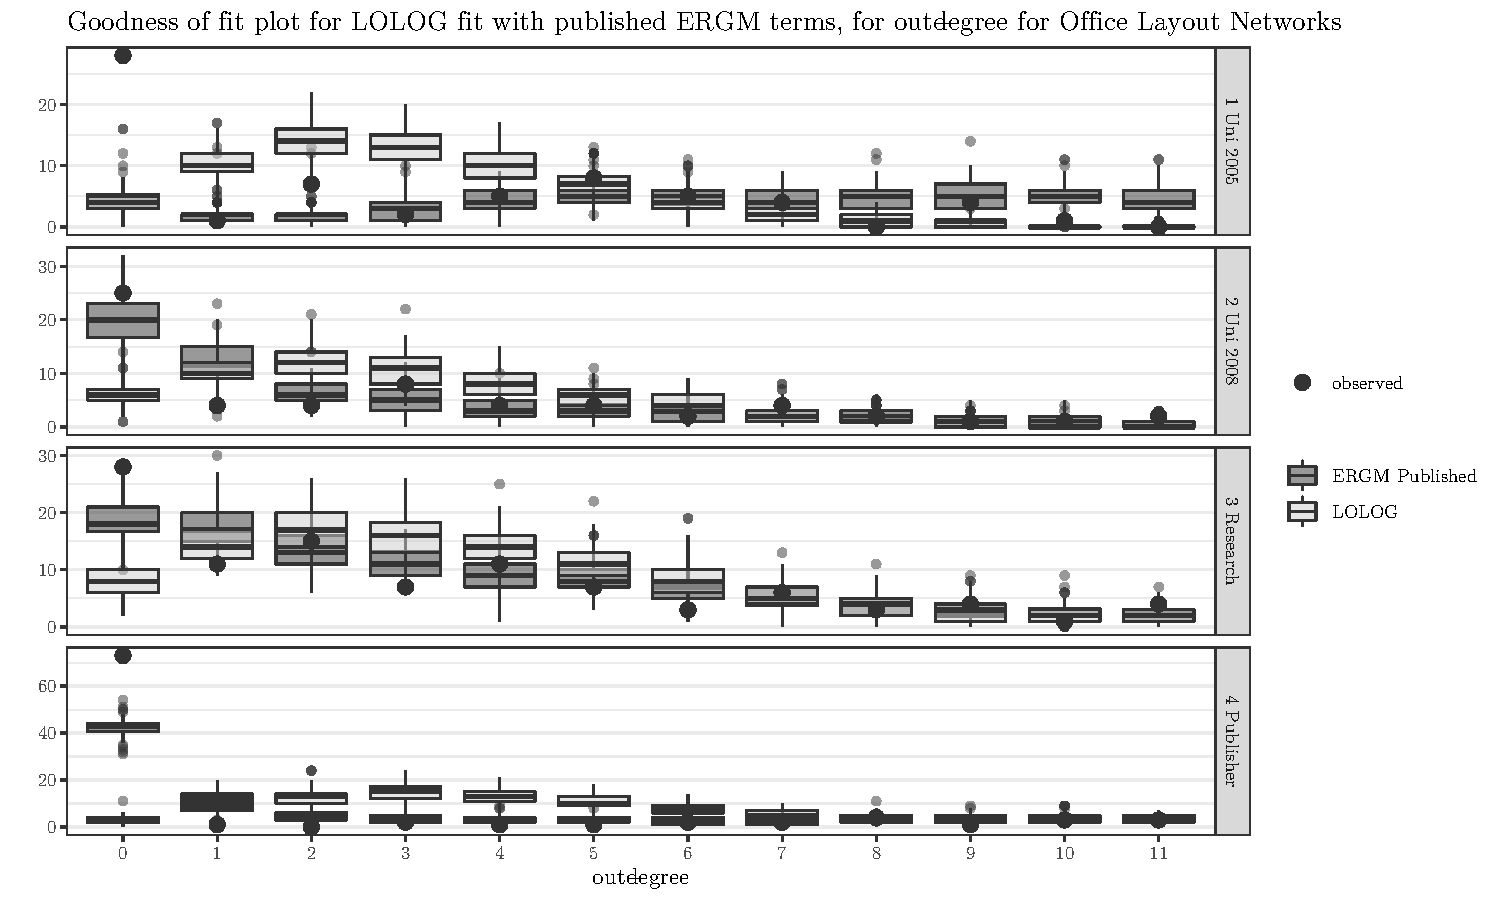
\includegraphics{lolog_catelog_writeup_JRSSA_major_revisions_git_files/figure-latex/unnamed-chunk-9-1} 

}

\caption{\label{fig:sailer_gof_pub_odeg} Sailer's Offices ERGM and LOLOG model with published terms, out-degree Goodness of Fit}\label{fig:unnamed-chunk-9}
\end{figure}

\begin{figure}[H]

{\centering 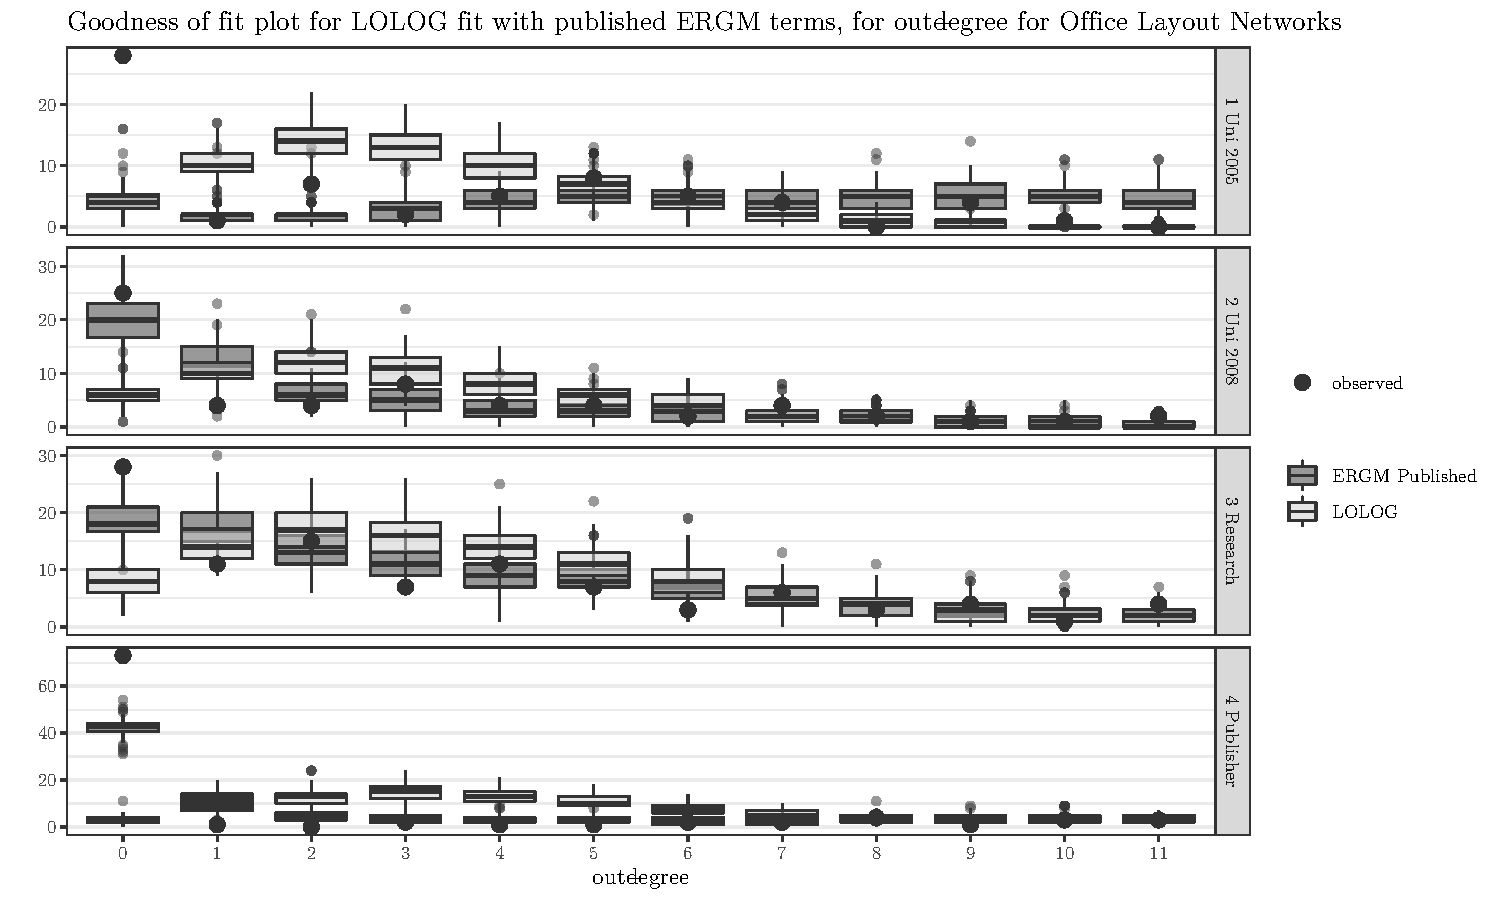
\includegraphics{lolog_catelog_writeup_JRSSA_major_revisions_git_files/figure-latex/unnamed-chunk-10-1} 

}

\caption{\label{fig:sailer_gof_pub_esp} Sailer's Offices ERGM and LOLOG model with published terms, ESP Goodness of Fit}\label{fig:unnamed-chunk-10}
\end{figure}

\begin{figure}[H]

{\centering 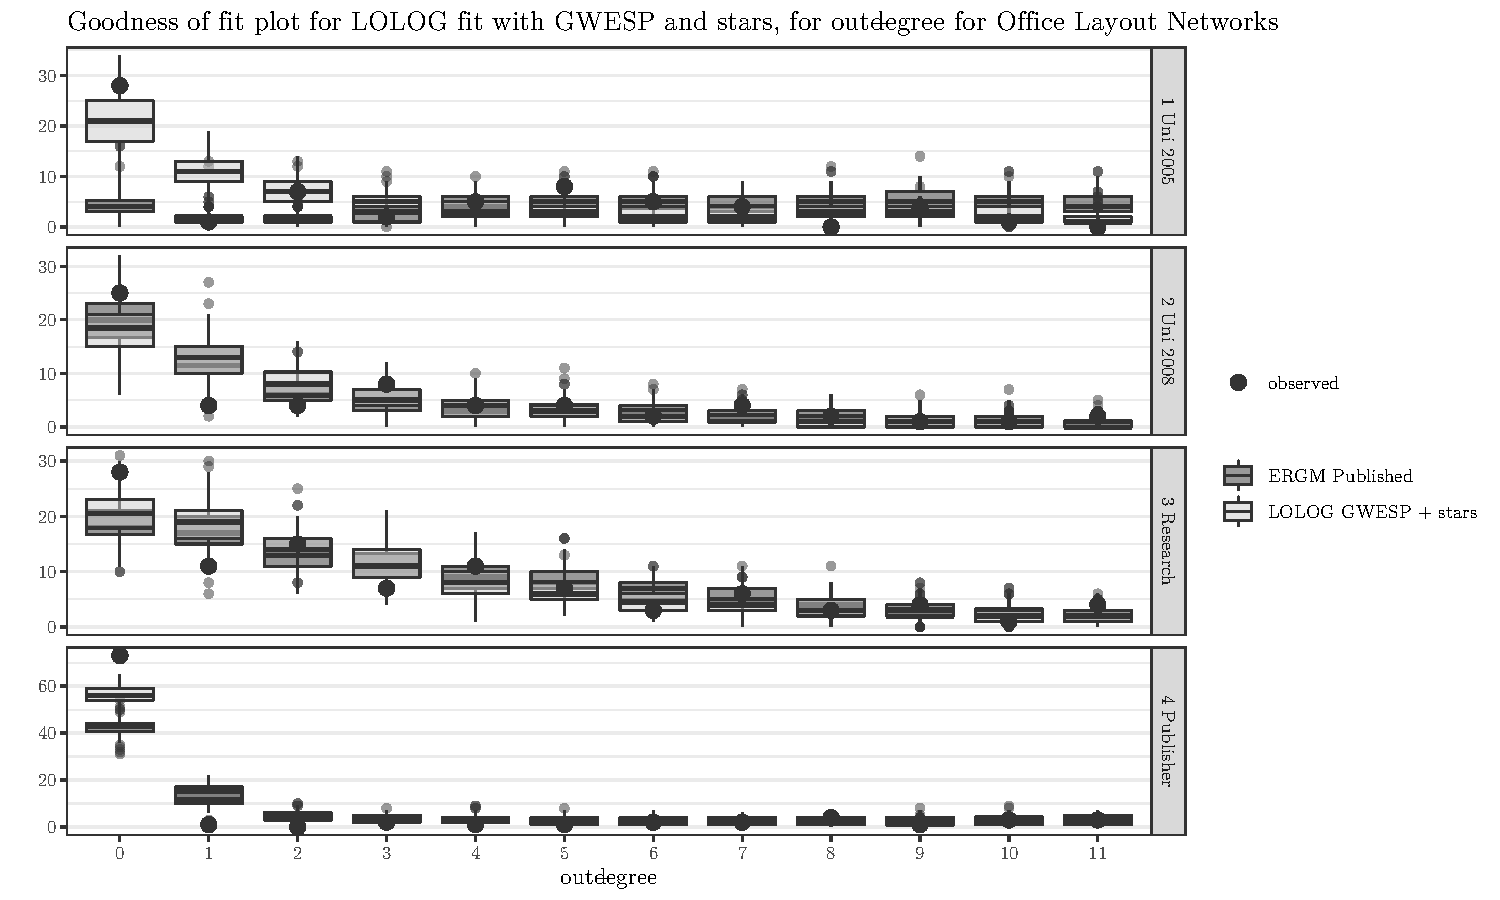
\includegraphics{lolog_catelog_writeup_JRSSA_major_revisions_git_files/figure-latex/unnamed-chunk-11-1} 

}

\caption{\label{fig:sailer_gof_gwesp_star_odeg} Sailer's Offices LOLOG model with GWESP and stars, out-degree Goodness of Fit}\label{fig:unnamed-chunk-11}
\end{figure}

\begin{figure}[H]

{\centering 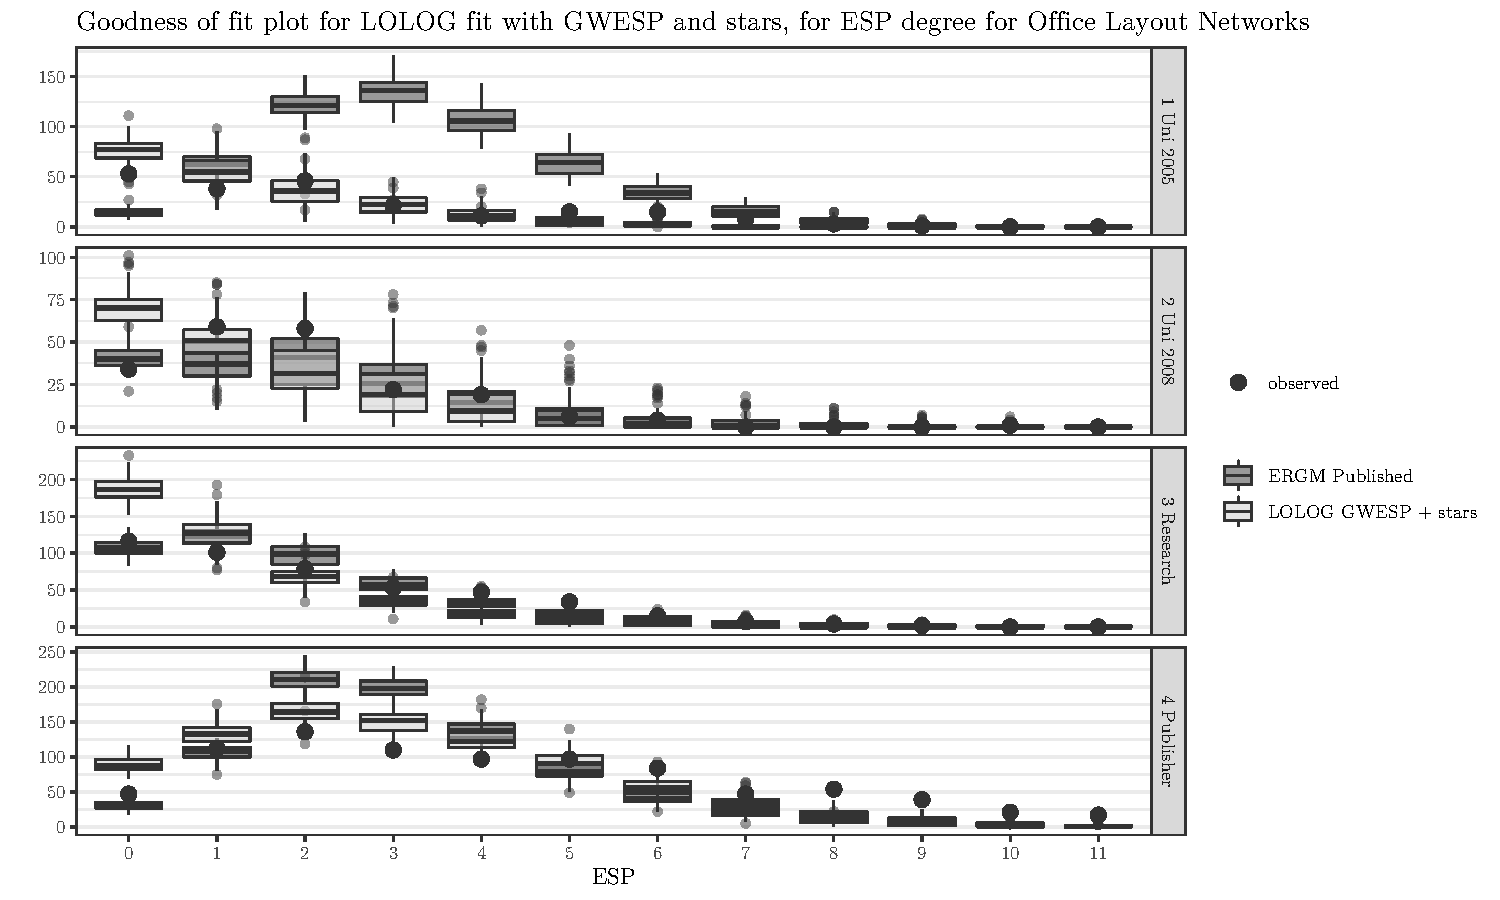
\includegraphics{lolog_catelog_writeup_JRSSA_major_revisions_git_files/figure-latex/unnamed-chunk-12-1} 

}

\caption{\label{fig:sailer_gof_gwesp_star_esp}Sailer's Offices LOLOG model with GWESP and stars, ESP Goodness of Fit}\label{fig:unnamed-chunk-12}
\end{figure}

\section{Links to publically available data}

Table \ref{tab:public_data} provides hyperlinks to the publicly
available datasets used in our ensemble.

\begin{longtable}[t]{ll}
\caption{\label{tab:unnamed-chunk-13}\label{tab:public_data} Links to publicly available datasets}\\
\toprule
Network & Links\\
\midrule
\rowcolor{gray!6}  Add Health & addhealth.cpc.unc.edu/\\
Elementary School & moreno.ss.uci.edu/data.html\#children\\
\rowcolor{gray!6}  Florentine Families & sites.google.com/site/ucinetsoftware/datasets/padgettflorentinefamilies\\
Kapferer's Tailors & sites.google.com/site/ucinetsoftware/datasets/kapferertailorshop\\
\rowcolor{gray!6}  Natural Disasters & vlado.fmf.uni-lj.si/pub/networks/data/GBM/kansas.htm\\
\addlinespace
German Schoolboys & github.com/gephi/gephi/wiki/Datasets\\
\rowcolor{gray!6}  Company Boards & corp.boardex.com\\
\bottomrule
\end{longtable}

\bibliographystyle{chicago}
\bibliography{bib}

\end{document}
